\documentclass[11pt,a4paper]{article}
\usepackage[margin=2.2cm]{geometry}
\usepackage{booktabs}
\usepackage{array}
\usepackage{graphicx}
\usepackage{subcaption}

\title{\textbf{Update Progress 11 September 2026}}
\date{}
\author{}

\begin{document}
\maketitle
\vspace{-1.5em}

\begin{figure}[h]
\centering
\begin{subfigure}{0.47\textwidth}
\centering
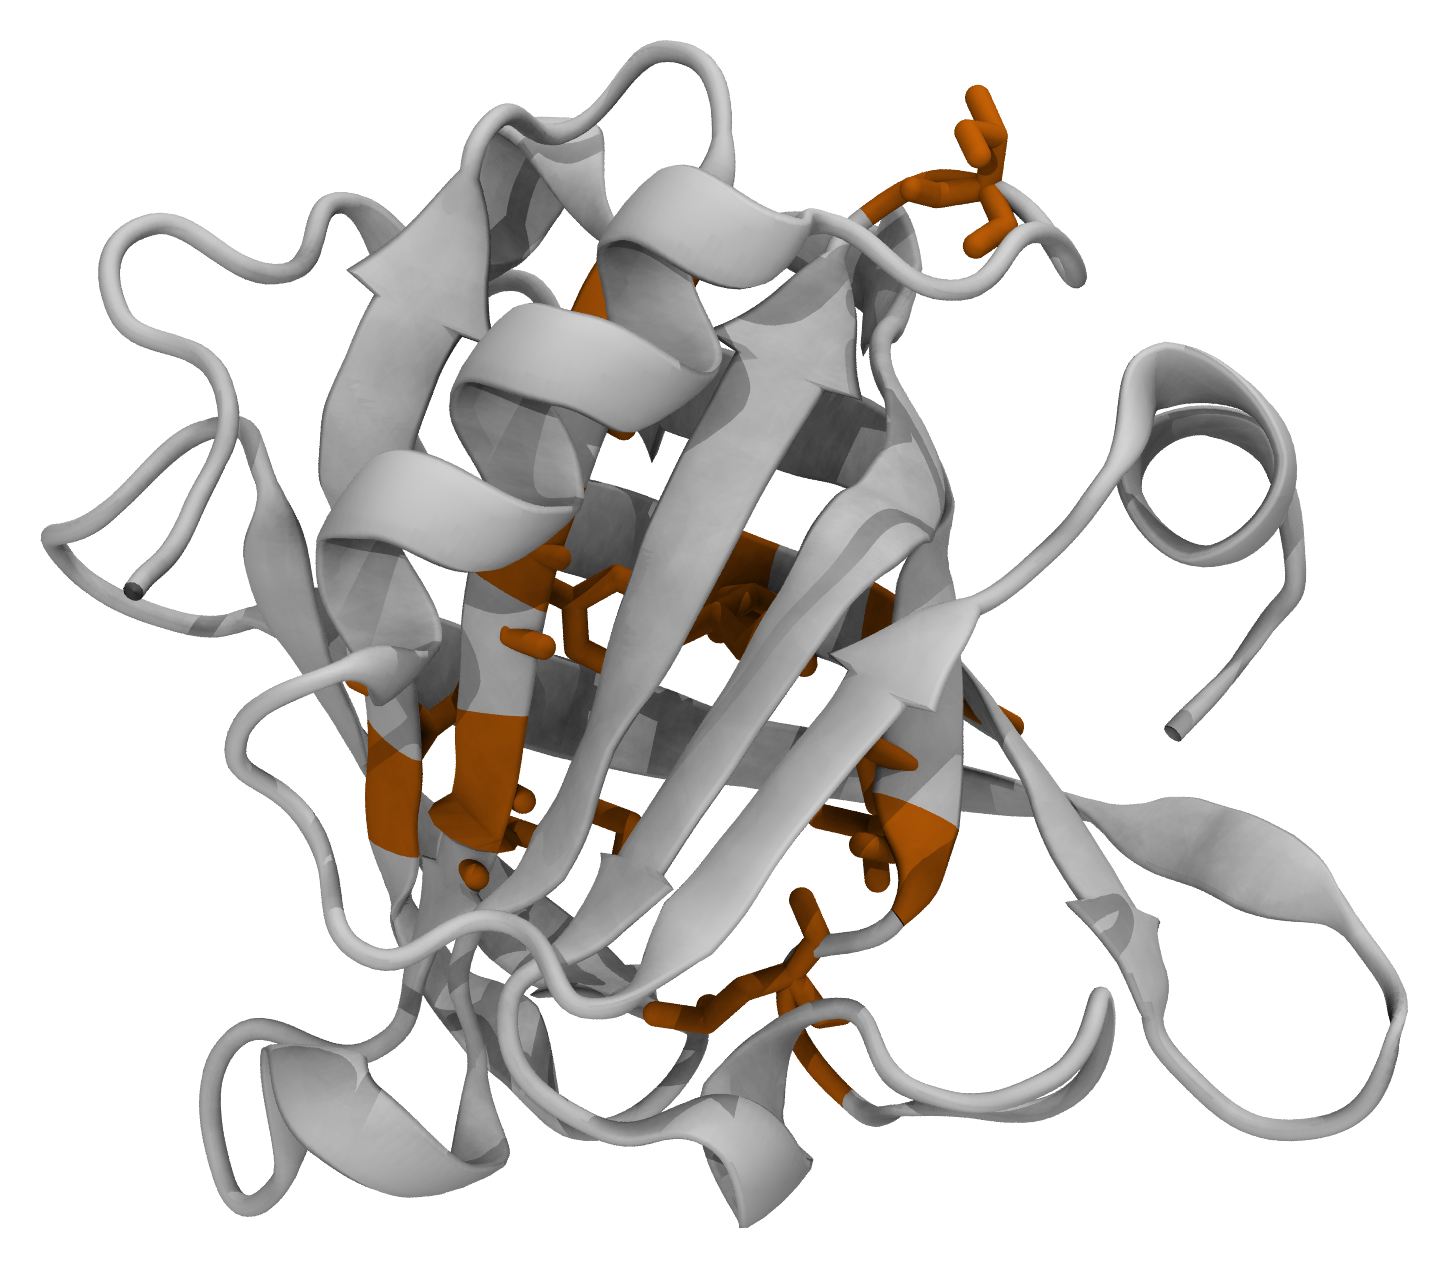
\includegraphics[width=\textwidth]{../results/figures/render/blg_calyx_crop.png}
\caption{BLG: compact fold, calyx patch (orange)}
\end{subfigure}
\hfill
\begin{subfigure}{0.47\textwidth}
\centering
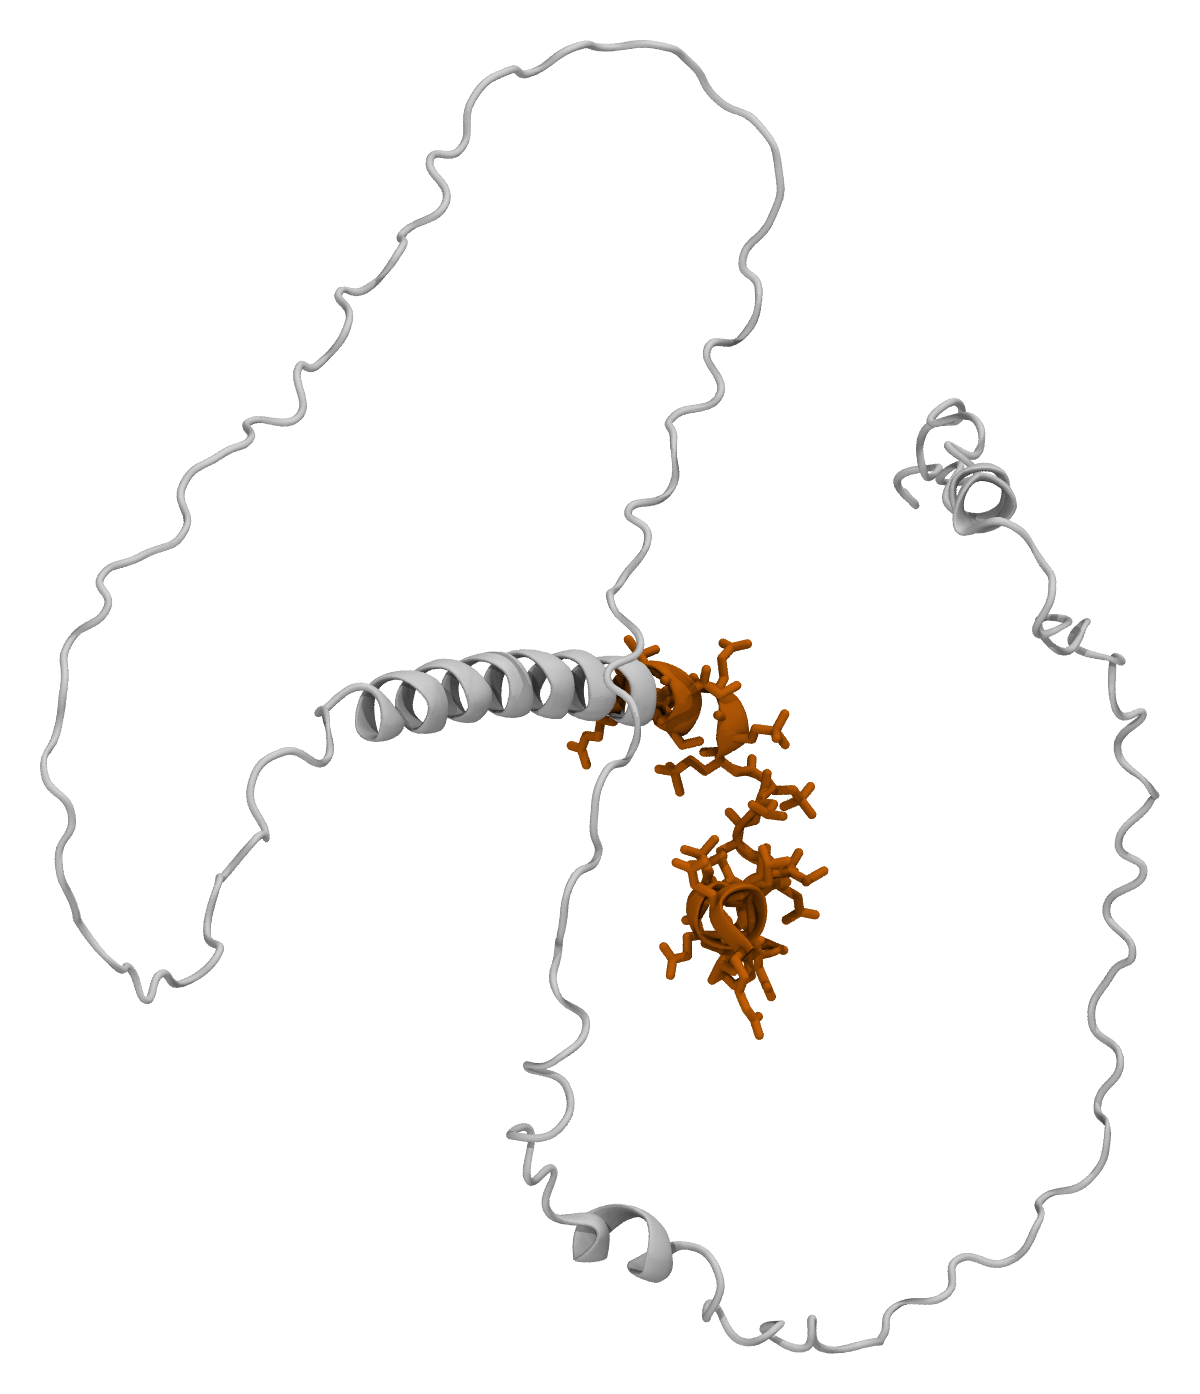
\includegraphics[width=\textwidth]{../results/figures/render/cas_patch_crop.png}
\caption{CASEIN: extended chain, N-term (orange)}
\end{subfigure}
\caption{\textbf{Structural contrast between the two proteins} (VMD renders): BLG's
compact, mostly-buried calyx vs. CASEIN's extended, disordered chain with its
N-terminal region already surface-exposed even in the starting structure.}
\end{figure}

\section{BLG Results}

\textbf{Headline numbers (unchanged, PBC-corrected, computed across all 4 replicas):} 613
total contact events (97 in CENTER, 516 near-interface across replicas); 6 long contact events
($\geq$10 ns); calyx SASA range 24--37 nm$^2$ (mean 28.95 nm$^2$); Pearson correlation between SASA
and orientation angle $r = +0.006$ (block-bootstrap 95\% CI $[-0.09, +0.11]$) -- no coupling detected
within these limits. These support the paper's current framing: BLG's calyx remains accessible
throughout, but the protein does not commit to a bound, reoriented state within the simulated
timescale.

\begin{table}[h]
\centering
\scriptsize
\setlength{\tabcolsep}{4pt}
\begin{tabular}{lccccc}
\toprule
Replica & $R_g$ (nm)$^*$ & RMSD bb (nm) & RMSD patch (nm) & Calyx SASA (nm$^2$) & $\gamma$ (mN/m)$^*$ \\
\midrule
CENTER (1000 ns) & 1.504 $\pm$ 0.022 & 0.229 & 0.198 & 3.81 $\pm$ 0.46 & 51.9 $\pm$ 38.5 \\
R1                & 1.497 $\pm$ 0.009 & 0.237 & 0.347 & 3.15 $\pm$ 0.34 & 52.7 $\pm$ 38.7 \\
R2                & 1.493 $\pm$ 0.008 & 0.206 & 0.254 & 3.59 $\pm$ 0.32 & 52.0 $\pm$ 39.0 \\
R3                & 1.499 $\pm$ 0.012 & 0.268 & 0.276 & 3.36 $\pm$ 0.48 & 52.6 $\pm$ 39.4 \\
\bottomrule
\end{tabular}
\normalsize
\caption{BLG per-replica structural summary. $^*$For R1/R2/R3, only $R_g$ and $\gamma$
(surface tension) currently reflect the first 500 of 1000 ns each replica actually ran
-- a fix to include the remaining trajectory segments for these two analyses is in
progress. RMSD and calyx SASA for R1/R2/R3 already cover the full 1000 ns (their
analysis scripts already include the extension trajectory segments).}
\end{table}

\begin{figure}[h]
\centering
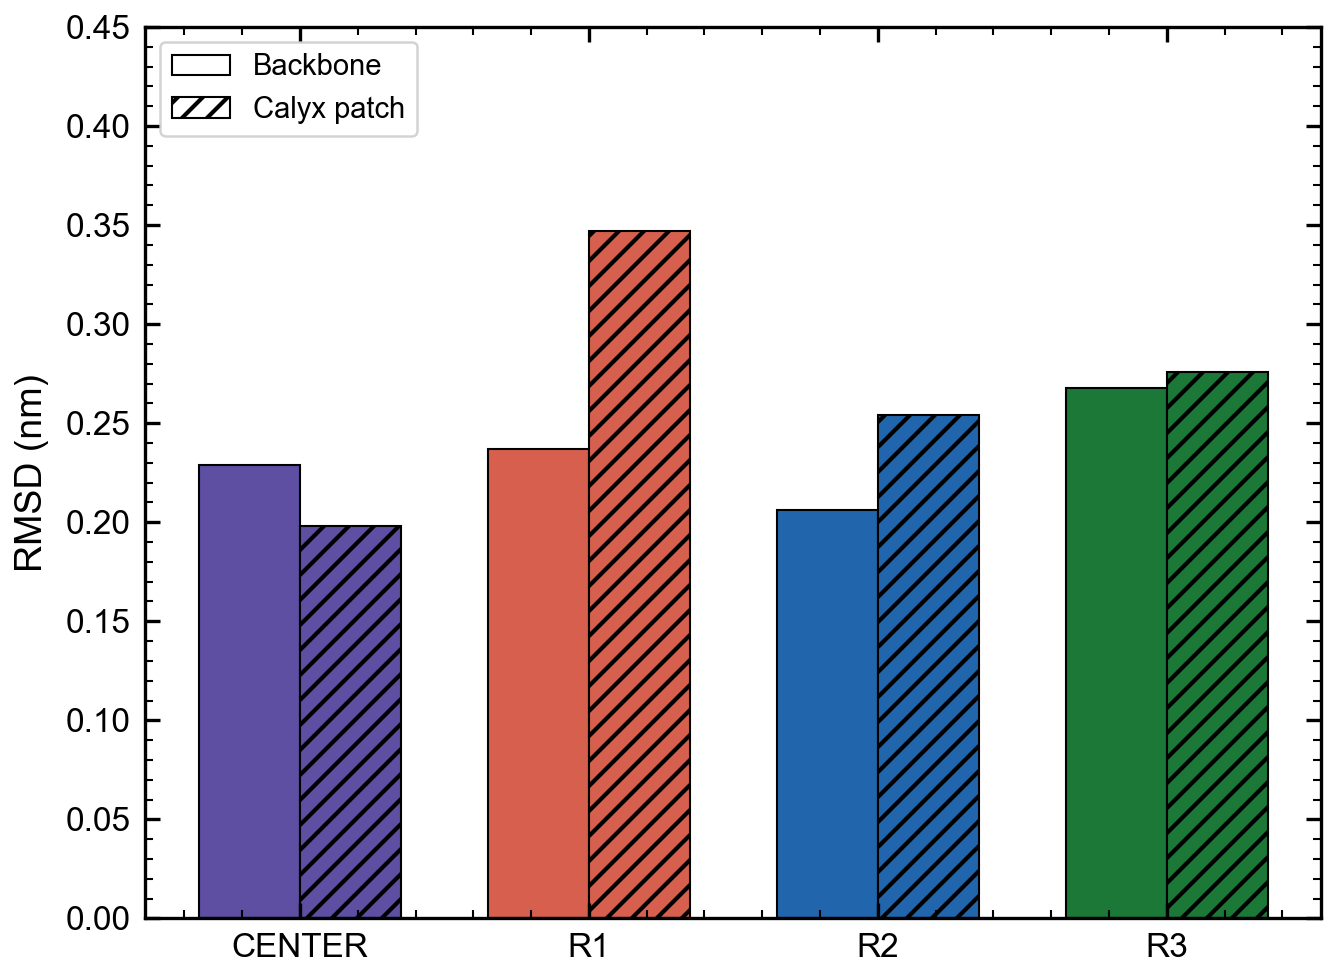
\includegraphics[width=0.6\textwidth]{../results/figures/paper/PAPER_COMPARATIVE_RMSD.png}
\caption{BLG RMSD by region, all 4 replicas: whole-backbone (solid) vs. calyx patch
(hatched). R1's patch RMSD is visibly elevated relative to the other replicas --
traced to a long ($\geq$10 ns) contact event unique to R1, not a bug.}
\end{figure}

\begin{figure}[h]
\centering
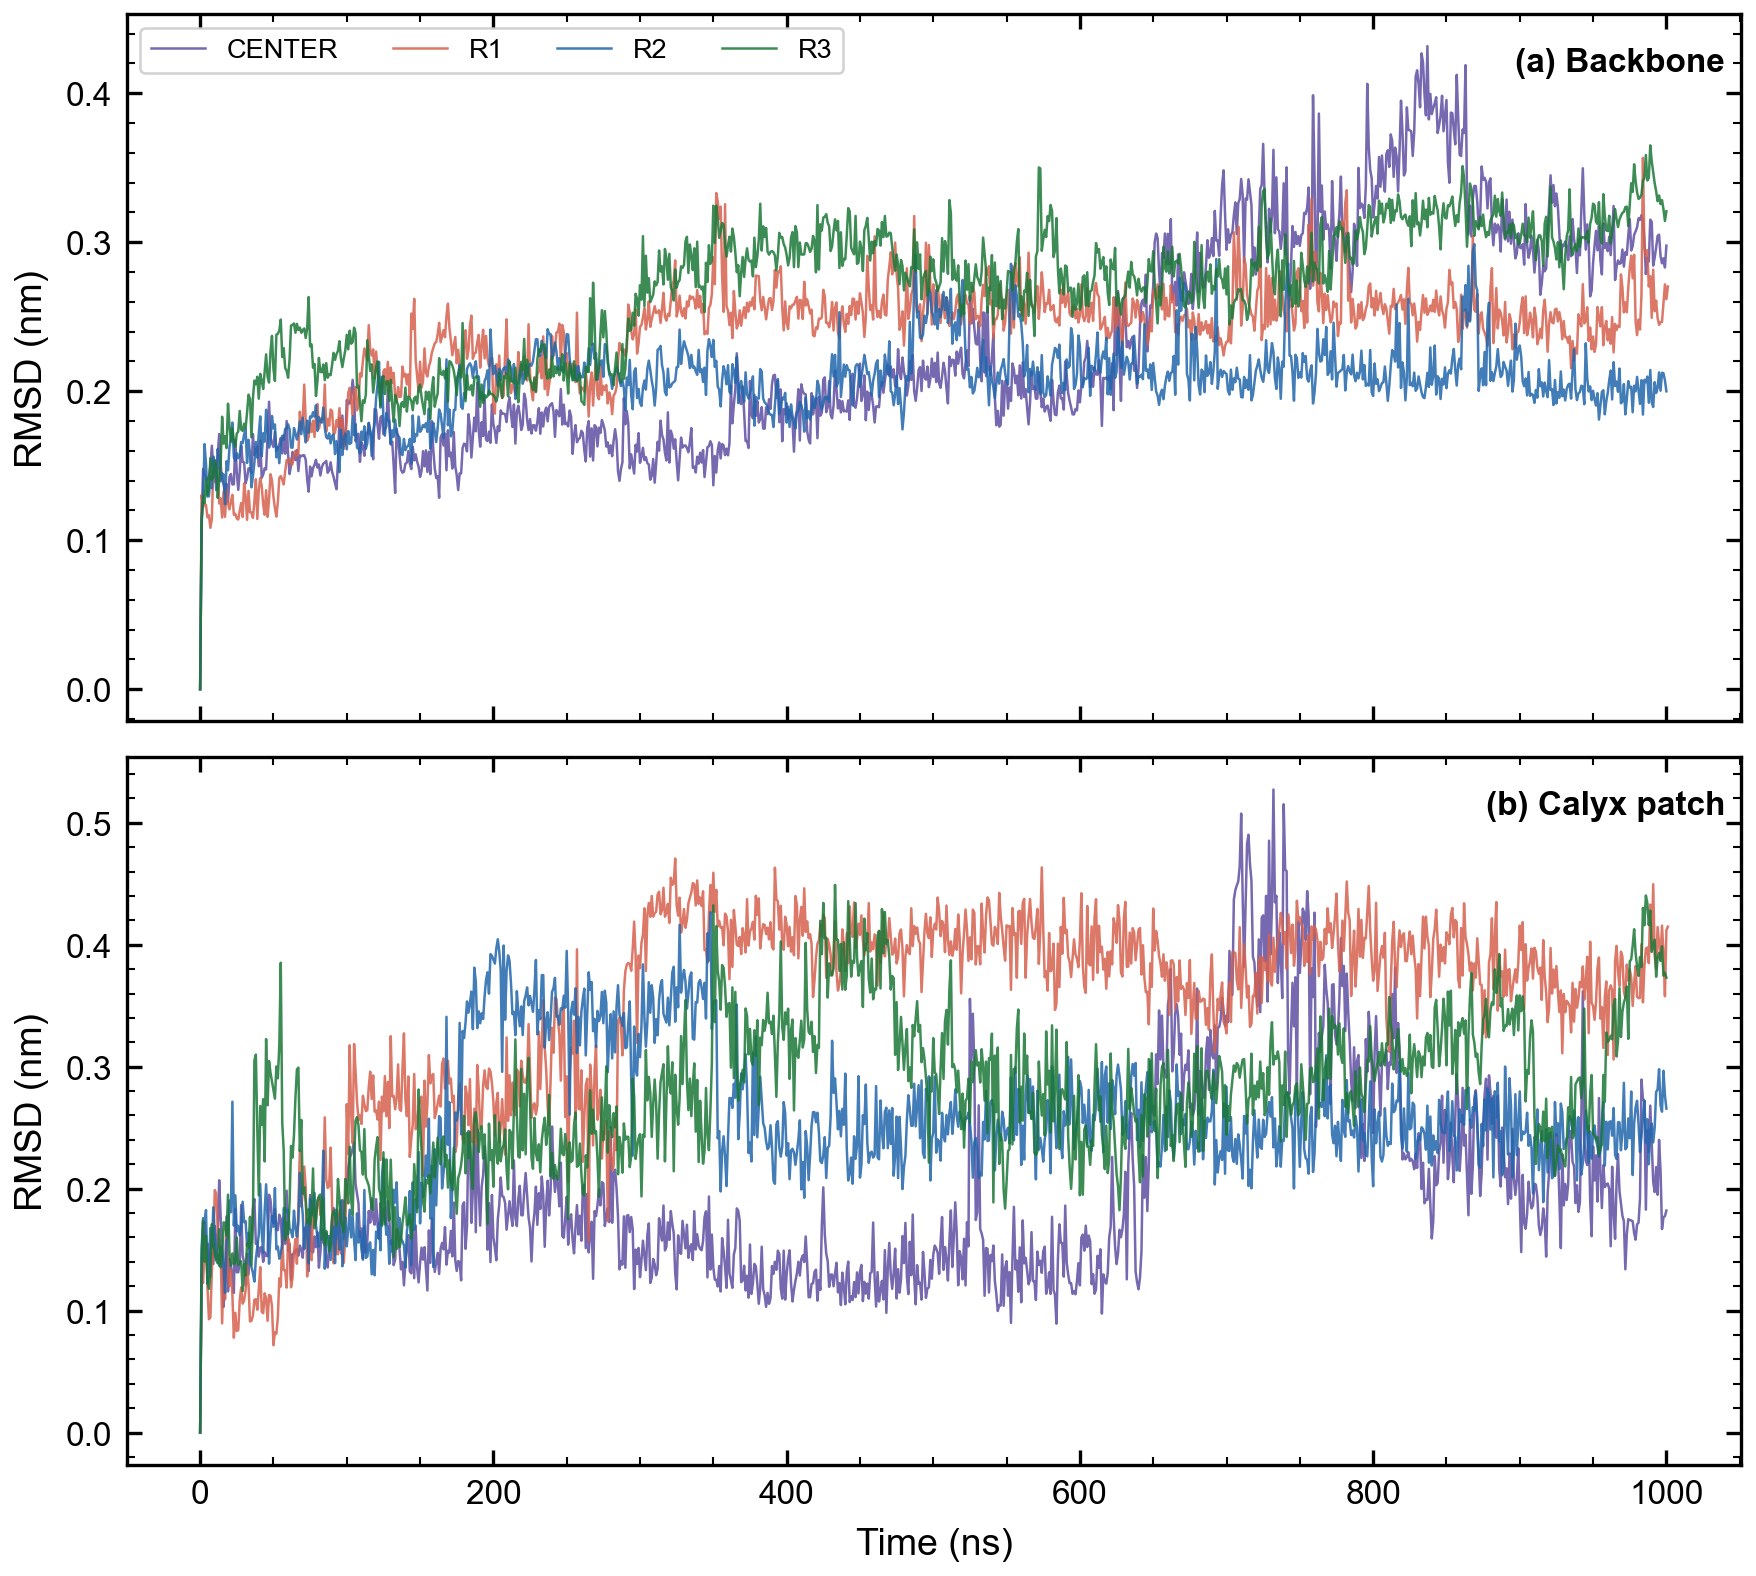
\includegraphics[width=0.85\textwidth]{../results/figures/paper/PAPER_TIMESERIES_RMSD.png}
\caption{BLG RMSD vs. time, all 4 replicas (backbone and calyx patch). The trend view:
R1's patch RMSD (orange, panel b) visibly steps up around 350 ns and never returns to
baseline -- the moment of its long contact event -- while CENTER's patch RMSD (purple)
stays lowest and flattest throughout.}
\end{figure}

Secondary structure content (DSSP) is stable across all 4 replicas: Helix 10.5--12.4\%,
Sheet 36.0--36.8\%, Coil 50.8--52.9\%. Hydrogen-bonding (CENTER only so far):
protein--protein 107.3 $\pm$ 5.6, protein--water 393.2 $\pm$ 13.2, interface
water--water 9539.6 $\pm$ 328.4 (mean counts per frame).

\section{CASEIN ($\beta$-casein) Results}

\textbf{First comparative result with real replication (n=2):} N-terminal region (residues
1--25) solvent accessibility -- the CASEIN analogue of BLG's calyx SASA -- is
24.77 $\pm$ 1.40 nm$^2$ in R1 vs. 25.41 $\pm$ 1.97 nm$^2$ in CENTER. The two independent
1000 ns runs agree closely, which is good evidence this is a real, reproducible property
of the protein rather than an artifact of one starting structure.

\begin{table}[h]
\centering
\scriptsize
\setlength{\tabcolsep}{4pt}
\begin{tabular}{lccccc}
\toprule
Replica & N-term SASA (nm$^2$) & Contact & $\gamma$ (mN/m) & Hbonds prot-prot & Hbonds prot-water \\
\midrule
CENTER (1000 ns) & 25.41 $\pm$ 1.97 & 99.5\% & 51.4 $\pm$ 34.2 & 97.8 $\pm$ 9.7 & 565.5 $\pm$ 25.1 \\
R1 (1000 ns)     & 24.77 $\pm$ 1.40 & 99.5\% & 52.4 $\pm$ 34.6 & 92.0 $\pm$ 8.3 & 575.9 $\pm$ 24.0 \\
\bottomrule
\end{tabular}
\normalsize
\caption{CASEIN per-replica summary. Both replicas now have all 7 planned analyses
complete. "Contact" is the fraction of frames with a protein-water minimum distance
$\leq$0.3 nm; R1 shows 1 sustained contact event across the full 1000 ns run.}
\end{table}

\begin{figure}[h]
\centering
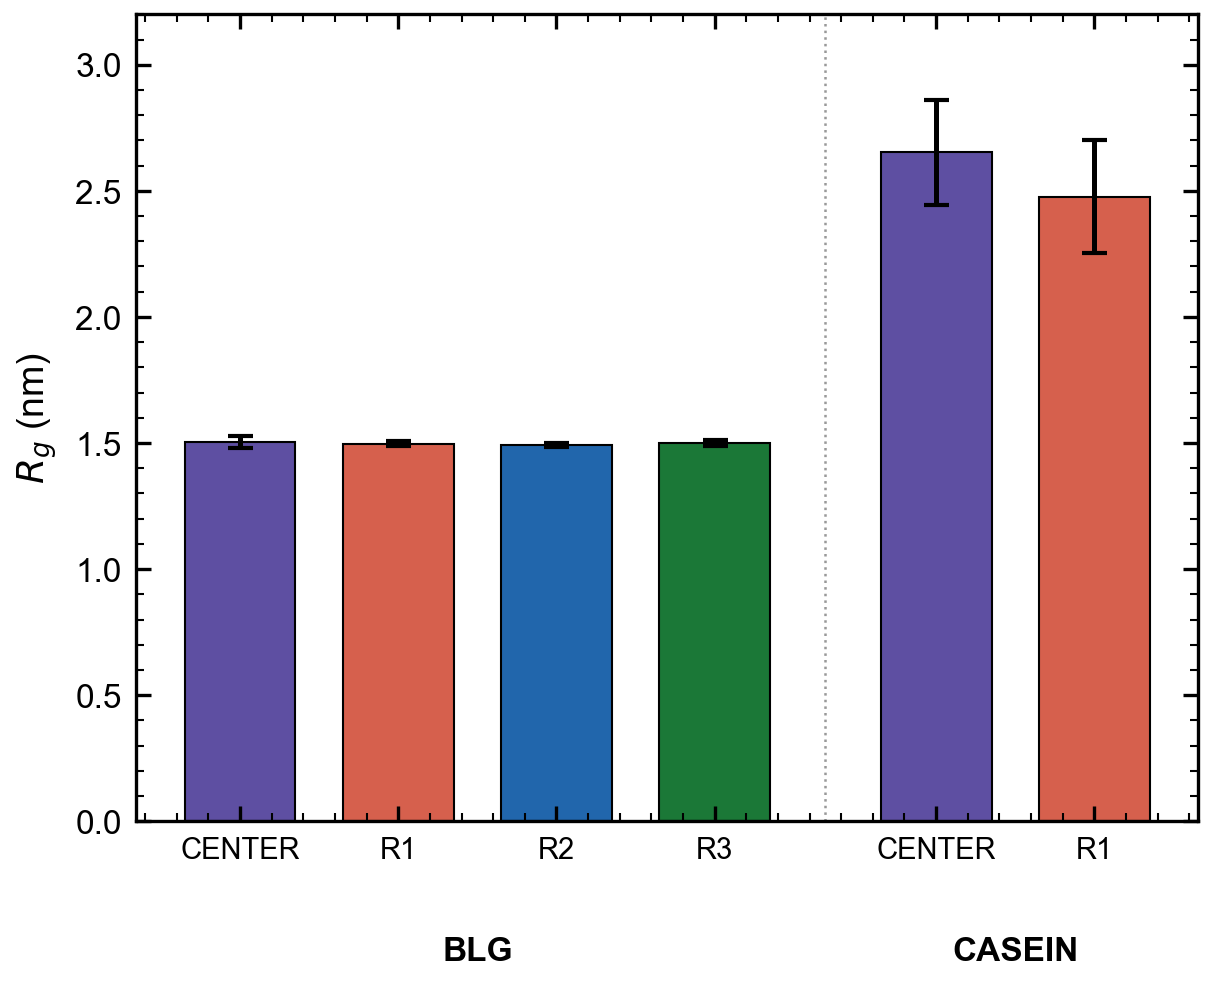
\includegraphics[width=0.6\textwidth]{../results/figures/paper/PAPER_COMPARATIVE_RG.png}
\caption{Radius of gyration, BLG vs. CASEIN, all replicas. BLG stays tightly compact
($\sim$1.5 nm, all 4 replicas) while CASEIN settles to a larger, still stable range
($\sim$2.5--2.7 nm) after its initial relaxation from an extended starting structure.}
\end{figure}

\begin{figure}[h]
\centering
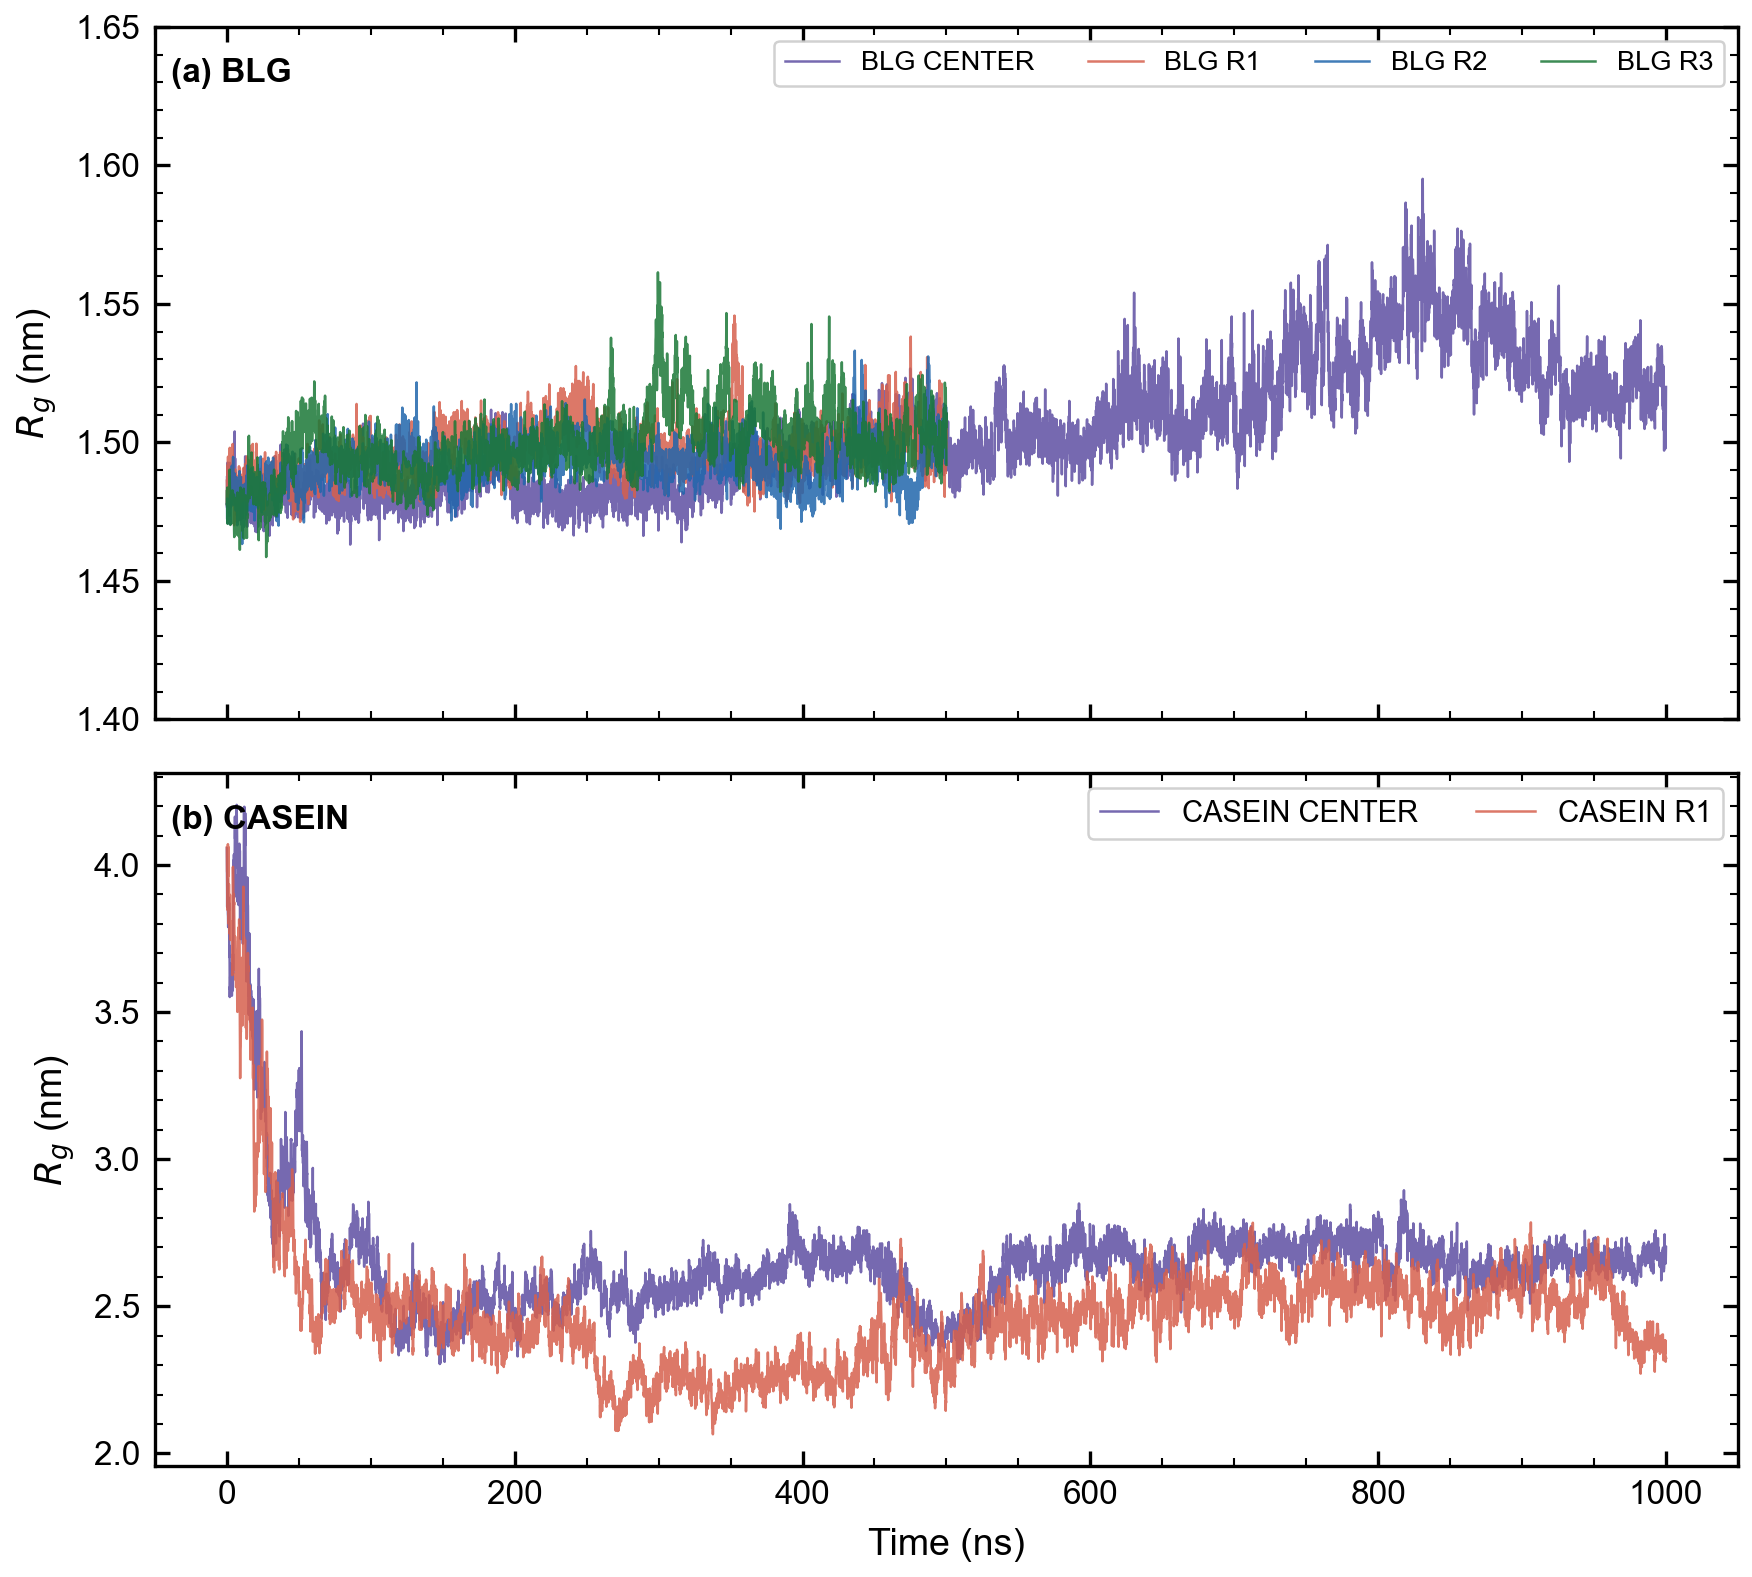
\includegraphics[width=0.85\textwidth]{../results/figures/paper/PAPER_TIMESERIES_RG.png}
\caption{$R_g$ vs. time. BLG (panel a) is flat and tightly clustered around 1.5 nm from
t=0 -- no relaxation needed, it started compact. CASEIN (panel b) starts extended
($\sim$4 nm, its AlphaFold starting structure) and visibly relaxes down to $\sim$2.5 nm
within the first $\sim$100 ns, then stays there -- the relaxation transient is directly
visible here, not just summarized as a mean.}
\end{figure}

\begin{figure}[h]
\centering
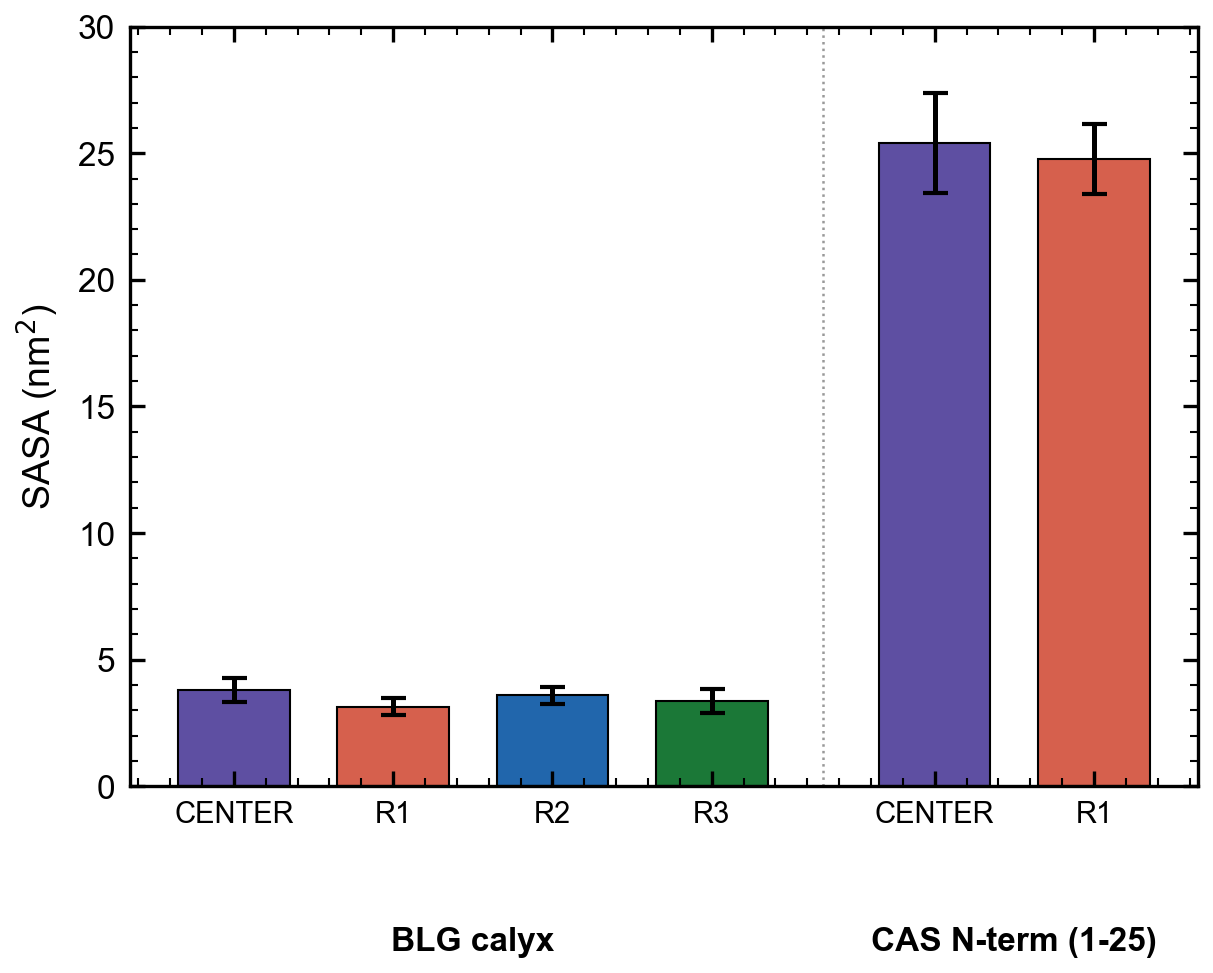
\includegraphics[width=0.78\textwidth]{../results/figures/paper/PAPER_COMPARATIVE_SASA.png}
\caption{Accessible surface area, BLG calyx vs. CASEIN N-terminal region (residues
1--25), all replicas. The $\sim$7-fold size difference is consistent across every
replica of both proteins -- not an artifact of any single run.}
\end{figure}

\begin{figure}[h]
\centering
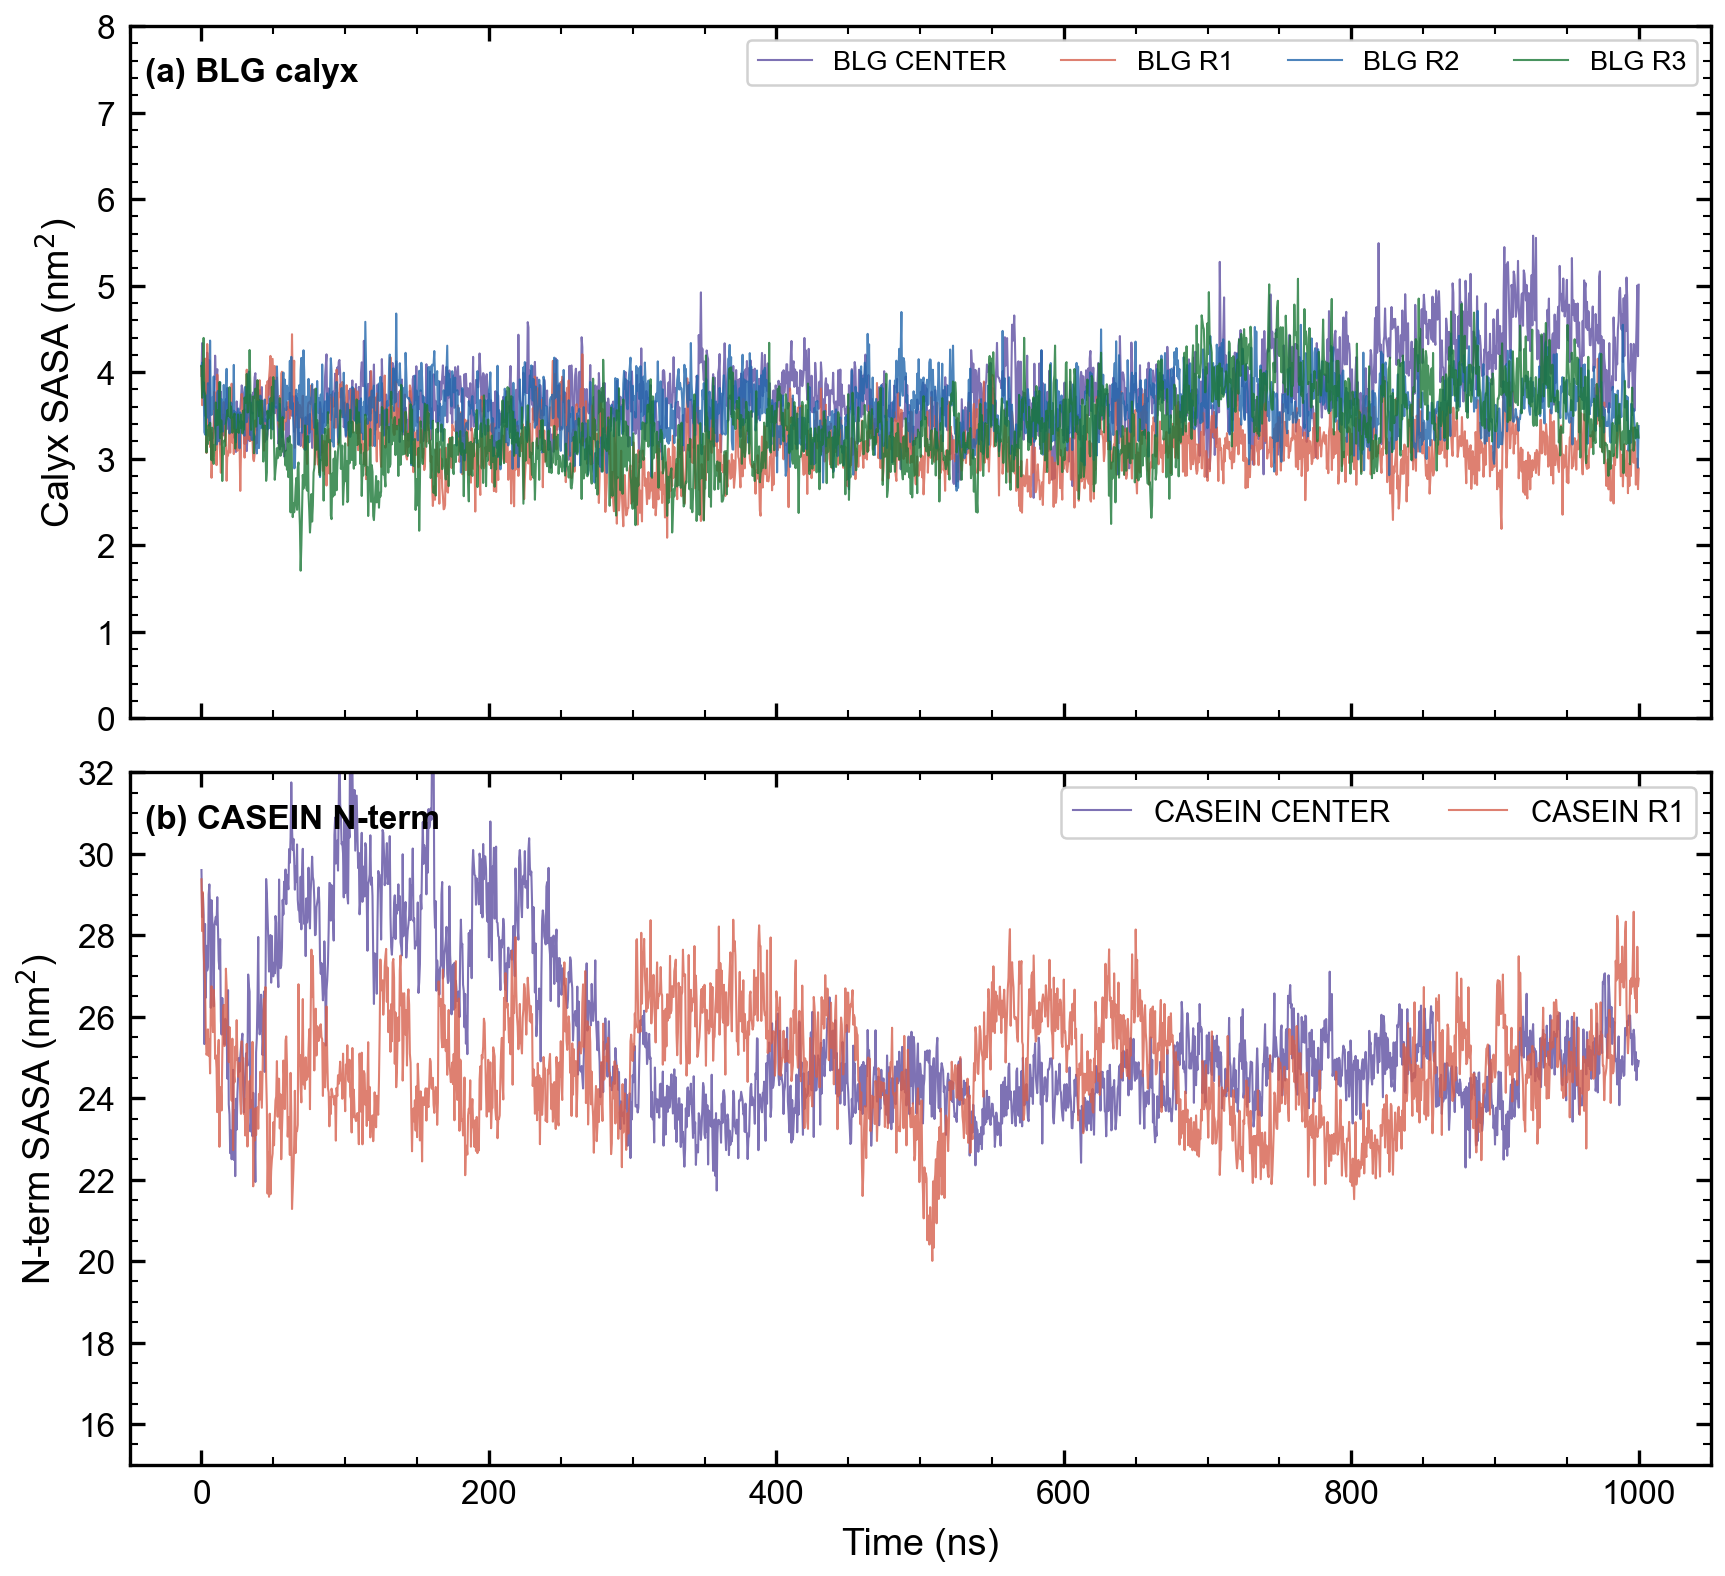
\includegraphics[width=0.85\textwidth]{../results/figures/paper/PAPER_TIMESERIES_SASA.png}
\caption{SASA vs. time. BLG's calyx (panel a) fluctuates in a narrow band ($\sim$2--5.5
nm$^2$) throughout, all 4 replicas overlapping closely. CASEIN's N-terminus (panel b)
fluctuates far more broadly (roughly 20--32 nm$^2$) but never drops anywhere near BLG's
range -- the size gap holds at every single timepoint, not just on average.}
\end{figure}

Hydrogen-bonding is also now complete for both replicas and agrees closely
(protein-protein 92.0--97.8, protein-water 565.5--575.9, interface water-water
12015.6--12750.5 mean counts per frame) -- another independent confirmation that
CENTER's behavior was not a one-off.

\begin{figure}[h]
\centering
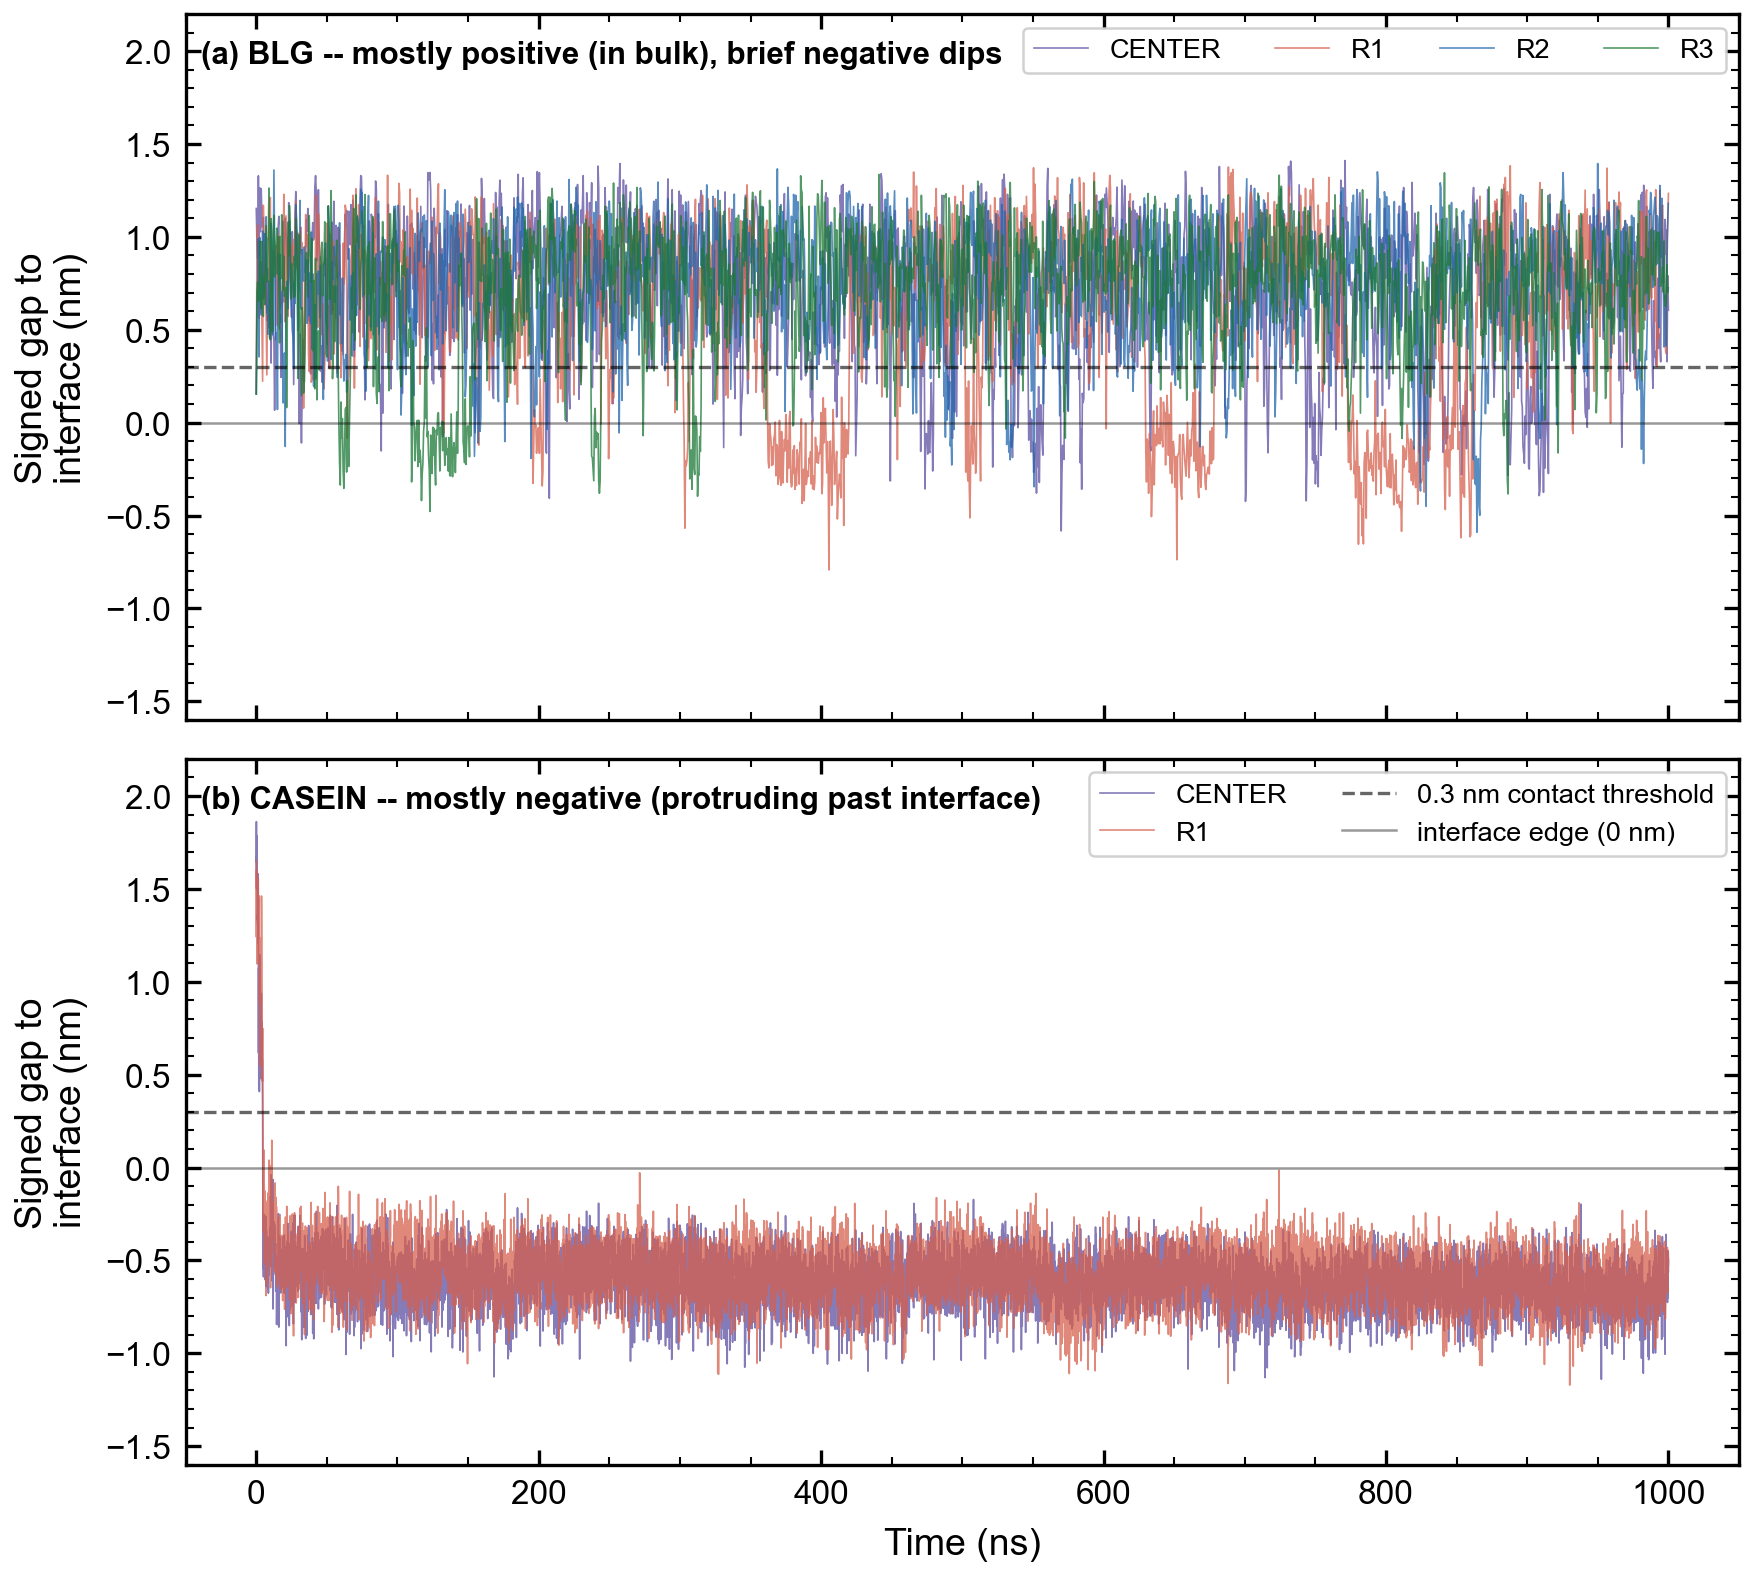
\includegraphics[width=0.85\textwidth]{../results/figures/paper/PAPER_TIMESERIES_CONTACT.png}
\caption{Signed protein-to-interface gap vs. time (positive = inside the water bulk,
negative = protruding past the water's statistical edge, into the interfacial/vacuum
region -- see caption note in the source script for the exact definition). BLG (panel
a) sits mostly positive with brief, distinct negative excursions -- these are its
613 discrete contact events. CASEIN (panel b) sits almost entirely negative
throughout both replicas, averaging around $-0.6$ nm -- it does not just touch the
interface, it persistently protrudes past it for virtually the whole trajectory.}
\end{figure}

\end{document}
